\subsection{Sensitivity to centering and correction labels}
\label{sec:implementation-sensitivity}
Two additional experiments examine the distinction between the training-row
kernel predictions and the predictor evaluated at a new input. First, we
rerun the six-member pipeline at the same ten seeds, changing only the
target mean used in each out-of-fold kernel fit. Both arms retrain the
kernel-conditioned refiner for 100 epochs and refit the stack and residual
correction; the remaining members are held fixed. Pooled centering gives
$\sensPooled\pm\sensPooledSd\%$ mean relative error and fold-local
centering gives $\sensLocal\pm\sensLocalSd\%$. The paired difference,
fold-local minus pooled, is $\sensCenterDelta\pm\sensCenterDeltaSd$
percentage points. Figure~\ref{fig:implementation-sensitivity} shows every
seed, including the direction of the change. This comparison isolates the
effect of target centering.

Second, we hold the stack weights and selected correction kernel
fixed, evaluate the query-time mean on the training rows, and replace the
correction labels by residuals of that mean. No network is retrained in this
check. The resulting test error is
$\sensConsistent\pm\sensConsistentSd\%$, a paired change of
$\sensMismatchDelta\pm\sensMismatchDeltaSd$ percentage points from the
original correction. The propagated mismatch
$\|c_\lambda(u)^\top\Delta\|_2/\|G(u)\|_2$ from
\eqref{eq:mismatch} averages
$\sensMismatchMean\pm\sensMismatchMeanSd\%$ across seeds and cases.
It measures the difference between two finite-design predictors.
Supplement~\ref{supp:sensitivity} gives the protocol, full stage comparisons,
and calibration results.

\begin{figure}[t]
\centering
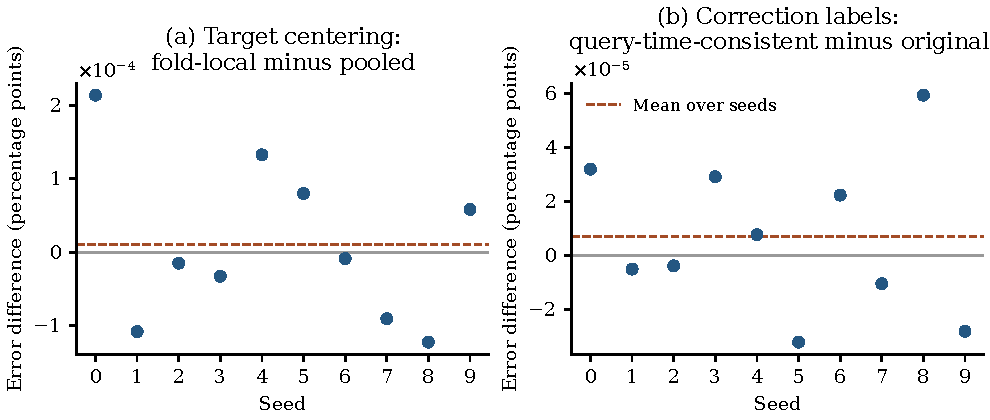
\includegraphics[width=\linewidth]{figs/paired_implementation_sensitivity.pdf}
\caption{Paired changes in mean relative test error for the ten mechanics
seeds. Left: fold-local minus pooled target centering, with downstream
refiner training and fitting repeated in both arms. Right: correction labels
consistent with the query-time mean minus the original labels, with the
mean and kernel fixed. Positive values mean higher error after the change.
The panels use separate vertical scales. All points use the same public
test block; the dashed lines are seed means.}
\label{fig:implementation-sensitivity}
\end{figure}
